%!TEX root =  main.tex
\chapter{Distributed computing}\label{chapter:Field_overview}
%
An overview of the distributed computing (DC) topics that are of significant importance for the rest of the thesis is going to be given in this section, since the thesis is heavily based on these topics. 

Sections~\ref{sec:distributed_systems} and \ref{sec:distributed_computing} describe the theoretical background behind the problem, where we examine distributed systems (DS) and distributed programming (DP), focusing on design details, communication patterns, and organizational structure. Section~\ref{sec:similar_models} describes similar models that might be a source of confusion, and how they are different than DS or DC, and how some concepts can fit in the bigger picture. Section~\ref{sec:transactions} describes different transaction models used for different applications. Section~\ref{sec:garbage_collection} describes basics of garbage collection techniques and why it is important. Section~\ref{sec:virtualization_techniques} describes different virtualization methods that are used in CC for systems and/or applications. Section~\ref{sec:deployment} describes different architecture and application model and how deployment can be done in large DS. Section~\ref{sec:ias} describes infrastructure as software model that allows abstracting infrastructure to software level. Section~\ref{sec:dev_roles} describes different development roles in the modern complex software environment, with focus on technical roles, while Section~\ref{sec:concurency_parallelism} describes the difference between concurrency and parallelism and introduces an actor system, that will be used later on in the thesis. 

\section{Distributed systems}\label{sec:distributed_systems}
%
There are various definitions of DS, but we can think of DS as a system where multiple entities can communicate to one another in some way, but at the same time, they can perform some operations. In~\cite{SteenT16, 0019513} Tanenbaum et al. give two interesting assumptions about DS:

\begin{enumerate}[start=1,label={(\bfseries \arabic*)}]
	\item  \say{A computing element, which we will generally refer to as a node, can be either a hardware device or a software process}.
	\item \say{A second element is that users (be they people or applications) believe they are dealing with a single system. This means that one way or another the autonomous nodes need to collaborate}.\label{ds:asumption_2}
\end{enumerate}

\noindent
These two assumptions are useful and powerful when talking about DS. As such, in this thesis, we will adopt and use them rigorously.

Three significant characteristics of distributed systems are~\cite{0019513}: 

\begin{enumerate}[start=1,label={(\bfseries \arabic*)}]
	\item \textbf{concurrency of components}, refers to the ability of the DS that multiple activities are executed at the same time. These activities take place on multiple nodes that are part of a DS.
	\item \textbf{independent failure of components}, this property refers to a nasty feature of DS that nodes fail independently. They can fail at the same time as well, but they usually fail independently for numerous reasons.
	\item \textbf{lack of a global clock}, this is a consequence of dealing with independent nodes. Each node has its notion of time, and as such we cannot assume that there is something like a global clock.
\end{enumerate} 

\noindent
In~\cite{SteenT16} authors give formal definition \say{distributed system is a collection of autonomous computing elements that appears to its users as a single coherent system}.

When talking about DS, we usually think about computing systems that are connected via network or over the internet. But DS is not exclusive to the domain of computer science. They existed before computers started to enrich almost every aspect of human life. DS have been used in various different domains such as: \textbf{telecommunication networks}, \textbf{aircraft control systems}, \textbf{industrial control systems} etc. DS are used anywhere where the number of users is growing rapidly so that a single entity cannot respond to the demands in (near) real-time.

Distributed systems (in computer science) consist of various algorithms, techniques, and trade-offs to create an illusion that a set of nodes act as one. Algorithms and techniques used in the DS may include the following: \textbf{(1)} replication, \textbf{(2)} consensus, \textbf{(3)} communication, \textbf{(4)} storage,\textbf{(5)} processing, \textbf{(6)} membership, \textbf{(7)} scheduling etc.

DS are hard to implement because of their asinchroninis and faulty nature. James Gosling and Peter Deutsch both fellows at Sun Microsystems at the time created a list of problems for network applications known as \textit{8 fallacies of Distributed Systems}~\cite{articleRotem}:\label{enum:fallacies}

\begin{enumerate}[start=1,label={(\bfseries \arabic*)}]\label{ds:8_fallacies}
	\item \textbf{The network is reliable}; there will always be something that goes wrong with the network --- power failure, a cut cable, environmental disasters, etc.
	\item \textbf{Latency is zero}; locally latency is not an issue, but it deteriorates very quickly when you move to the internet and CC scenarios;
	\item \textbf{Bandwidth is infinite}; even though bandwidth is constantly getting better and better, the amount of data we try to push through it rise as well.
	\item \textbf{The network is secure};  Internet attack trends are showing growth, and this becomes a problem even more in public CC;
	\item \textbf{Topology doesn't change}; network topology is usually out of user control, and network topology changes constantly for numerous reasons --- added or removed new devices, servers, breaks, outages, etc;
	\item \textbf{There is one administrator}; nowadays there are numerous administrators for web servers, databases, cache and so on, , and companies collaborate with other companies or CC providers;
	\item \textbf{Transport cost is zero}; we have to serialize information and send data over the wire, which takes resources and adds to the total latency. The problem here is not just latency, but that information serialization takes time and resources;
	\item \textbf{The network is homogeneous}; today, a homogeneous network is the exception, rather than a rule. We have different servers, systems, clients that interact. The implication of this is that we have to assume interoperability between these systems sooner or later, which we must be aware of. We might also have some proprietary protocols that might also take time to send on and they may stay without support, so we should avoid them.
\end{enumerate}

\noindent
These fallacies were introduced over a decade ago, and more than four decades since we started building DS, but the characteristics and underlying problems remain pretty the same. An interesting fact is that even designers, architects still assume that technology solves everything. This is not the case in DS, and these fallacies should not be forgotten. Because of these problems, DS are hard to implement correctly and they are hard to maintain and test properly.
%
%
\subsection{Scalability}\label{sec:scalability}
%
Scalability is the property of a system to handle a growing amount of work by adding resources to the system~\cite{Bondi00}. When talking about computer systems, scalability can be represented in two ways:

\begin{itemize}
	\item \textbf{Scaling vertically} means upgrading the hardware that computer systems are running on --- adding mode CPU, RAM, storage. Vertical scaling can increase performance to what the latest hardware can offer, and here we are limited by the laws of physics and Moor's law \cite{Gustafson2011}. A typical example that requires this type of scaling is a relation database server. These capabilities are insufficient for moderate to big workloads.
	\item \textbf{Scaling horizontally} means that we scale our system by adding more and more computers, rather than upgrading the hardware of a single one. With this approach, we are (almost) limitless on how much we can scale. Whenever performance degrades we can simply add more computers (or nodes). These nodes are not required to be some high-end machines.
\end{itemize}

\noindent
Figure~\ref{fig:fig23} show difference betweeen scaling vertically and horizontally.

\begin{figure}[H]
	\begin{center}
		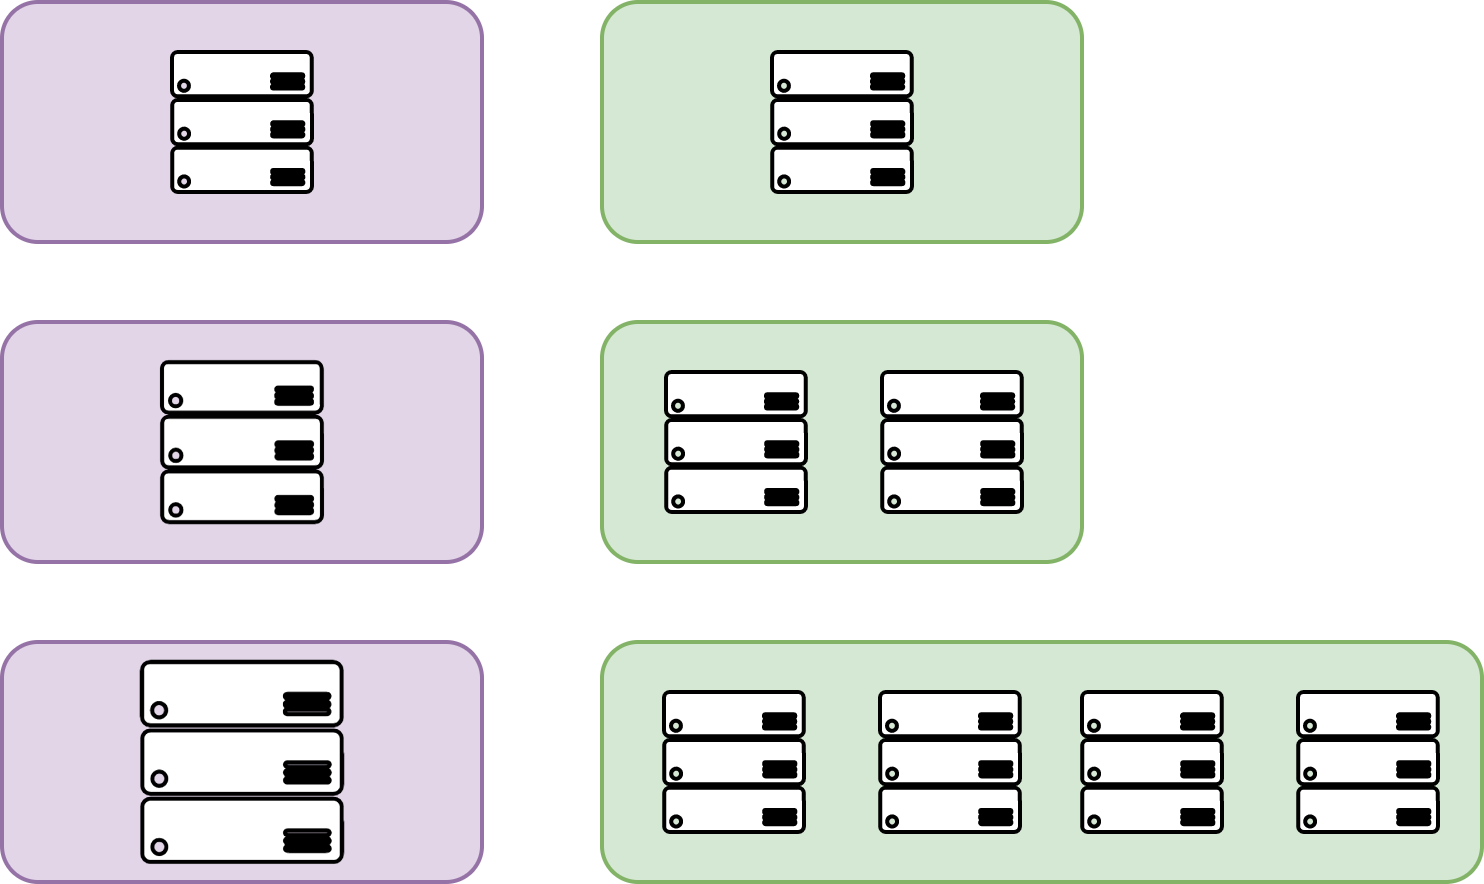
\includegraphics[scale=0.80]{images/Figure23}
	\end{center}
	\vspace{-0.6cm}
	\caption{Difference betweeen scaling vertically and horizontally}
	\label{fig:fig23}
\end{figure}

\noindent
Table~\ref{tab:table1} summarizes differences between horizontall and verticall scaling.

\begin{table}[h!]
	\begin{center}
		\begin{tabular}{l|l|l}
			\textbf{Feature} & \textbf{Scaling vertically} & \textbf{Scaling horizontally}\\
			\hline
			\textbf{Scaling} & Limited & Unlimited \\
			\textbf{Managment} & Easy & Comlex\\
			\textbf{Investments} & Expensive & Afordable \\
		\end{tabular}
	\end{center}
	\vspace{-0.5cm}
	\caption{Differences between horizontal and vertical scaling.}
	\label{tab:table1}
\end{table}

\noindent
Scaling horizontally is a preferable way for scaling DS. Not because we can scale easier, or because it is significantly cheaper than vertical scaling (after a certain threshold)~\cite{Bondi00}, but because this approach comes with few more benefits that are especially important when talking about large-scale DS. Adding more nodes gives us two important properties: 

\begin{itemize}
	\item \textbf{Fault tolerance} means that applications running on multiple places at the same time are not bound to the fail of a node, cluster, or even DCs. As long as there is a copy of the application running somewhere, the user will get a response back. As a consequence of running multiple copies of a service and on multiple places, we have that service is more \textbf{available}, than running on a single node no matter how high-end that node is. Eventually, all nodes are going to break, and if we have multiple copies of the same service we have a more resilient and more available system to serve user requests.
	\item \textbf{Low latency} refers to the idea that the world is limited by the speed of light. If a node running application is too far away, the user will wait too long for the response to get back. If the same application is running in multiple places, the user request will hit the node that is closest to the user.
\end{itemize}

\noindent
Nodes are usually organized into clusters of machines. Buyya et al. describes a cluster as a processing system, which consists of a collection of interconnected stand-alone computers cooperatively working together as a single, integrated computing resource.~\cite{Buyya}.

But despite all the obvious benefits, for a DS to work properly, we need the writing software in such a way that is able to run on multiple nodes, as well as that it \textbf{accepts the failure and deals with it}. This turns out to be not an easy task.

For example, users need to be aware when using DS which of them is related to distributed data storage systems. Storage implementations that rely on vertical scaling to ensure scalability and fault tolerance, have one nasty feature. 

This nasty feature is represented in theorem called \textbf{CAP theorem}~\label{lab:cap} presented by Eric Brewer~\cite{Brewer2000}, and proven after inspection by Gilbert et a.~\cite{GilbertL02}. The CAP theorem states that it is impossible for a distributed data store to simultaneously provide more than two out of three guarantees shown in Figure~\ref{fig:fig17}.

\begin{figure}[H]
	\begin{center}
		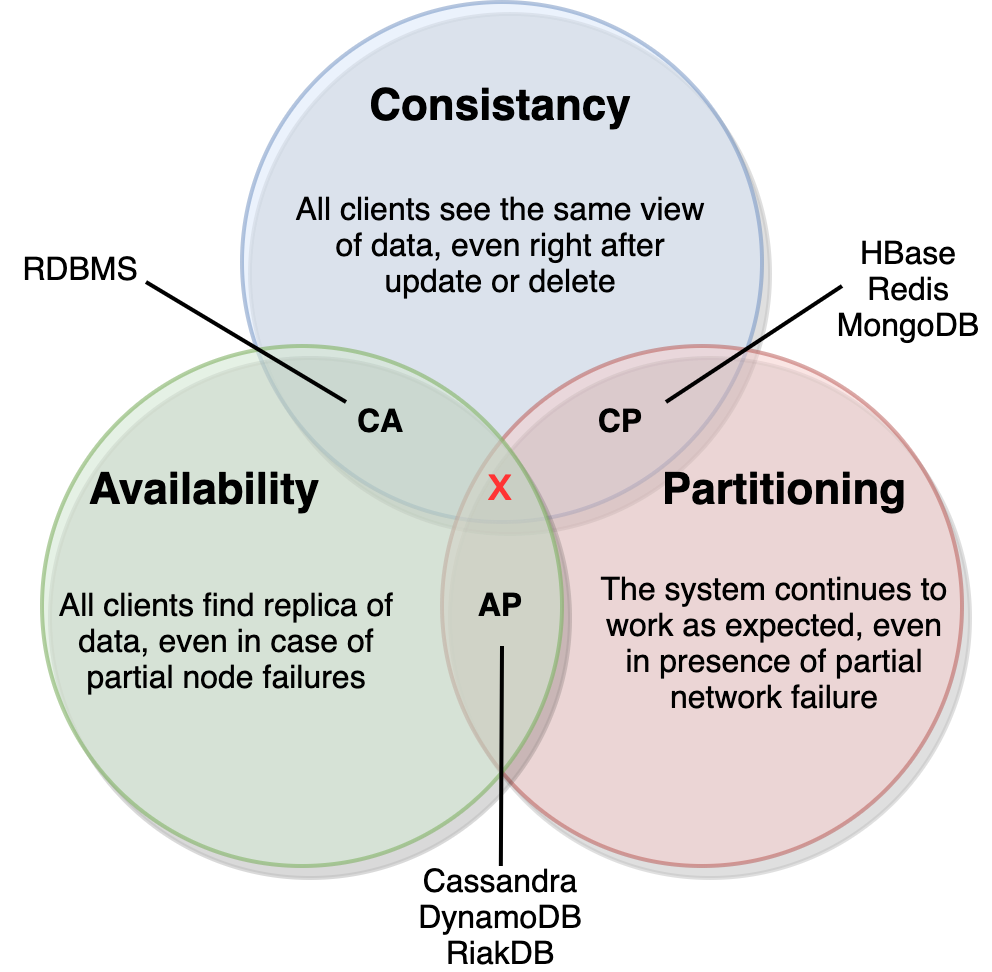
\includegraphics[scale=0.85]{images/Figure17}
	\end{center}
	\vspace{-0.6cm}
	\caption{Difference between cloud options and on-premises solution.}
	\label{fig:fig17}
\end{figure}

\begin{enumerate} [start=1,label={(\bfseries \arabic*)}]
	\item \textbf{C}onsistency, which means that all clients will see the same data at the same time, no matter which node they are connected to. Clients may not be connected to the same node since data could be replicated on many nodes in different locations.
	\item \textbf{A}vailability, which means that any client issued request will get a response back, even if one or more nodes are down. DS will not interpret this situation as an exception or error. Availability is represented in percentage, and it describes how much downtime is allowed per year. This can be calculated using formula:\\ 
	
	\begin{equation}\label{eq:Availability}
	Availability = \frac{uptime}{ (uptime + downtime)}
	\end{equation}
	\myequations{Availability percentage formula}
	The industry is using measuring availability in \say{class of nines}. Availability class is the number of leading nines in the availability figure for a system or module~\cite{GrayS91}. This metric relates to the amount of time (per year) that service is up and running. Table~\ref{tab:table7} show different classes of nine and their availability and unavailability in minutes per year (\textbf{min/year}) for some examples~\cite{GrayS91}.
	
	\begin{table}[h!]
		\begin{center}
			\begin{tabular}{l|l|l}
				\textbf{Type} & \textbf{Availability} & \textbf{Unavailability} \\
				\hline
				\textbf{Unmanaged} & 90\% & 50,000 \\
				\textbf{Managed} & 99\% & 5,000 \\
				\textbf{Well-managed} & 99.9\% & 500 \\
				\textbf{Well-managed} & 99.9\% & 500 \\
				\textbf{Fault-tolerant} & 99.99\% & 50 \\
				\textbf{High-availability} & 99.999\% & 5 \\
				\textbf{Very-high-availability} & 99.9999\% & 0.5 \\
			\end{tabular}
		\end{center}
		\vspace{-0.5cm}
		\caption{Downtime for different classes of nines.}
		\label{tab:table7}
	\end{table}
	
	\noindent
	We can calculate availability class if we have system availability $A$, the system's availability class is defined as~\cite{GrayS91}: 
	
	\begin{equation} 
	e^{\log_{10} \frac{1}{ (1 - A)}} 
	\end{equation}
	\myequations{Availability class formula.}
	It is important to notice that even a 99\% available system gives almost four days of downtime in a year, which is unacceptable for services like Facebook, Google, AWS, etc. And when the service is down, companies are losing customers.
	\item \textbf{P}artition tolerance, which means that the cluster must continue to work despite any number of communication breakdowns between nodes in the system. It is important to state that in a distributed system, partitions cannot be avoided.
\end{enumerate}

\noindent
Years after CAP theorem inception, Shapiro et al. prove that we can alleviate CAP theorem problems, but only in some cases, and offers \textbf{Strong Eventual Consistency (SEC) model}~\cite{ShapiroPBZ11}. They prove that if we can represent our data structure to be: \label{crdts}

\begin{itemize}
	\item \textbf{Commutative} $a*b = b*a$ \myequations{Commutative formula.}
	\item \textbf{Associative} $(a*b)*c = a*(b*c)$ \myequations{Associative formula.}
	\item \textbf{Idempotent} $(a * a) = a$ \myequations{Idempotent formula.}
\end{itemize}

\noindent
where $*$ is a binary operation, for example: $max$, $union$, $or$ we can rely on SEC properties,
%
%
\subsection{Cloud computing}\label{sec:cloud_computing}
%
Vogels et al. describe CC as an \say{aggregation of computing resources as a utility, and software as a service}~\cite{Vogels}.  Big DCs provide hardware and software services for their users over the internet~\cite{AboveTheCloud}. Cloud providers offer various resources like CPU, GPU, storage, and network as utilities that can be used and released on-demand~\cite{ZhangCB10}. 

The key strength of the CC is reflected in the offered services~\cite{Vogels}. To support the various application needs, the traditional CC model provides enormous computing and storage resources elastically. This property refers to the cloud ability to allow services to allocate additional resources or release unused ones to match the application workloads on-demand~\cite{AssuncaoVB18}. 

Services usually fall in one of three main categories: 

\begin{itemize}
	\item \textbf{Infrastructure as a service (IaaS)} allows businesses to purchase resources on-demand and as-needed instead of buying and managing hardware themselves;
	\item \textbf{Platform as a service (PaaS)} delivers a framework for developers to create, maintain and manage their applications. All resources are managed by the enterprise or a third-party vendor;
	\item \textbf{Software as a service (SaaS)} delivers applications over the internet to its users. These applications are managed by a third-party vendor;
\end{itemize}

\noindent
Figure~\ref{fig:fig1} shows the difference in control and management of resources between different cloud options and on-premises solutions.

\begin{figure}[H]
	\begin{center}
		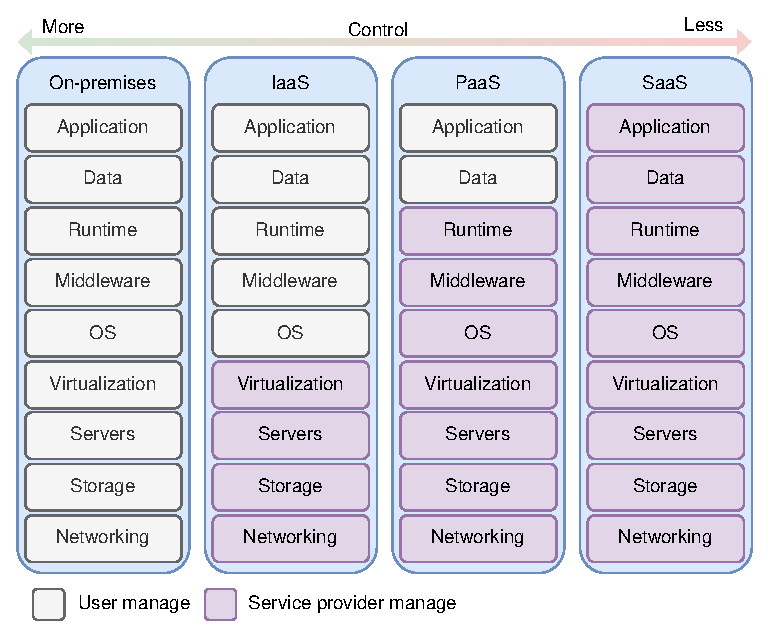
\includegraphics[scale=0.80]{images/Figure1}
	\end{center}
	\vspace{-0.6cm}
	\caption{Difference between cloud options and on-premises solution.}
	\label{fig:fig1}
\end{figure}

\noindent
The user can choose a single solution, or combine more of them if such a thing is required depending on preferences and needs.

By the ownership, CC can be categorized into three categories:

\begin{itemize}
	\item \textbf{Public cloud} is a type where CC is delivered over the internet and shared across many many organizations and users. In this type of CC, architecture is built and maintained by others. Users and organizations pay for what they use. Examples include AWS EC2, Google App Engine, Microsoft Azure, etc.
	\item \textbf{Private cloud} is a type where CC is dedicated only to a single organization. In this type of CC, architecture is built by an organization that may offer their solution or services to the users or other organizations. These services are in the domain of what the organization does, and that organization is in charge of maintenance. Examples include VMWare, XEN, KVM, etc.
	\item \textbf{Hybrid cloud} is such an environment that uses both public and private clouds. Examples include IBM, HP, VMWare vCloud, etc.
\end{itemize}

\noindent
Table~\ref{tab:table4} shows comparison of public, private and hybrid cloud capabilities.\label{sec_types}

\begin{table}[h!]
	\begin{center}
		\begin{tabular}{l|l|l|l}
			\textbf{Capabilities} & \textbf{Public cloud} & \textbf{Private cloud} & \textbf{Hybrid cloud}\\
			\hline
			\textbf{Data control} & IT enterprise & Service Provider & Both \\
			\textbf{Cost} & Low & High & Moderate \\
			\textbf{Data security} & Low & High & Moderate \\
			\textbf{Service levels} & IT specific & Provider specific & Aggregate \\
			\textbf{Scalability} & Very high & Limited & Very high \\	
			\textbf{Reliability} & Moderate & Very high & Medium/High\\	
			\textbf{Performance} & Low/Medium & Good & Good \\
		\end{tabular}
	\end{center}
	\vspace{-0.5cm}
	\caption{Comparison of public, private and hybrid cloud capabilities.}
	\label{tab:table4}
\end{table}

\noindent
In the rest of the thesis, if not stated differently when CC term is used it denotes public cloud.

CC has been the dominating tool in the past decade in various applications~\cite{Satyanarayanan17}. It is changing, evolving, and offering new types of services. Resources such as container as a service (CaaS), database as a service (DBaaS)~\cite{Peter} are newly introduced. The CC model gives us a few benefits. Centralization relies on the economy of scale to lower the cost of administration of big DCs. Organizations using cloud services avoid huge investments, like creating and maintaining their own DCs. They consume resources usually created by others~\cite{Satyanarayanan17} and pay for usage time -- pay as you go model. 

Centralization gives us a few really hard problems to solve. As already stated in section~\ref{sec:problem_area} data is required to be moved to the cloud from data sources, which introduces a high latency in the system~\cite{HossainRH18}. 

There are a few notable attempts to help data ingestion into the cloud. Remote Direct Memory Access (RDMA) protocol makes it possible to read data directly from the memory of one computer and write that data directly to the memory of another. This is done by using \textit{specialized hardware} interface cards and switches and software as well, and operations like read, write, send, receive, etc. do not go through the CPU. With these characteristics, RDMA has low latencies and overhead, and as such reaches better throughputs~\cite{CohenTKCKRCDG09}. This new hardware may not be cheap, and not every CC provider uses them for every use-case. This may not be enough, especially with the ever-growing amount of IoT devices and services.

Over the years there are more service options available, forming \textbf{everything as a service (XaaS)} model~\cite{DuanFZSNH15}. This model proposes that any hardware or software resource can be offered as a service to the users over the internet.

Table~\ref{tab:table2} shows common examples of SaaS, PaaS, and IaaS applications.

\begin{table}[h!]
	\begin{center}
		\begin{tabular}{l|l}
			\textbf{Platform} & \textbf{Common Examples}\\
			\hline
			\textbf{IaaS} & AWS, Microsoft Azure, Google Compute Engine \\
			\textbf{PaaS} & AWS Elastic Beanstalk, Azure, App Engine \\
			\textbf{SaaS} & Gmail, Dropbox, Salesforce, GoToMeeting \\
		\end{tabular}
	\end{center}
	\vspace{-0.5cm}
	\caption{Common examples of SaaS, PaaS, and IaaS.}
	\label{tab:table2}
\end{table}

\subsubsection{Multi-cloud and sky computing}
%
In recent years there has been one extension of CC from a series standpoint called \textbf{multi-cloud}~\cite{HongDSH19, Ardagna15} or sky computing~\cite{StoicaS21} (terms are going to be used interchangeably). 

It is such an environment where an enterprise uses more than one cloud platform, with at least two or more public cloud providers that each delivers a specific application or service. 

A multi-cloud can be comprised of any model presented on page~\pageref{sec_types}. This model relies on the possibility that if one cloud provider fails for whatever reason, the next one will be able to serve user requests.

This strategy allows creation of a single heterogeneous architecture, allowing distribution of cloud assets and workloads across multiple providers (active-active), or deploy a single workload on one provider, with a backup on another (active-passive)~\cite{Multicloud2019}.

CC gives a user an illusion that he is using a single machine, while the background implementation is fairly complicated and consists of various elements that are composed of countless machines. CC is a typical example of a horizontally scalable system presented in~\ref{sec:scalability}.
%
%
\subsection{Membership protocol}\label{sec:memership_protocol}
%
At the beginning of this section DS were introduced, and two interesting assumptions by Tanenbaum et al. were presented~\cite{SteenT16, 0019513}. If one more look is taken at~\ref{ds:asumption_2} assumption, we will see that users of the DS whether they are users or applications perceive DS as a single unit. Inside this single unit, nodes need to collaborate, so that they are able to do various kinds of tasks.

The most basic of all these tasks is that nodes need to know which group they belong to, and who are their peers in the group they will collaborate with. This might sound like a trivial idea, but when we include 8 fallacies of the DS~\ref{ds:8_fallacies} into the equation, things start to be not so trivial after all. In the setup where nodes are connected over the local network or internet, and they need to communicate, things will go wrong for various reasons.

To resolve the problem who their group peers are, a membership protocol comes to help. These protocols need to ensure that each process of one group updates its local list of \textbf{non-faulty} members of the group, and when a new process joins or leaves the group, the local list for every process needs to be updated. This is the most basic idea behind membership protocols.

Processes in the group of nodes in a group will ping each other in different ways, and using different strategies to figure out which nodes are dead and which are alive. There are a few existing algorithms that do this job, and they are (usually) based on the way epidemics spread or how gossip is spread in a human population. Because of this feature, these algorithms are usually called \textit{Gossip} style protocols.

Every membership protocol has some properties that will ensure efficiency and scalability:

\begin{enumerate}[start=1,label={(\bfseries \arabic*)}] \label{ds:features}
	\item \textbf{Completeness}, this property must ensure that every failure in the system is detected.
	\item \textbf{Accuracy}, in an ideal world, there should be no mistakes when detecting failures, but In a real-life scenario, we need to reduce false positives as much as we can.
	\item \textbf{Failure detection speed}, all failures needs to be treated as fast as possible, in order to remove the node from the group and reschedule the tasks from the dead node to alive ones.
	\item \textbf{Scale}, with this property we must ensure that the network load that is generated should be distributed equally between all processes in the group.
\end{enumerate}

\noindent
The easiest idea to implement this protocol would be \textbf{heartbeating} technique where process $P_i$ will send a heartbeat message to all his peers in the group or \textbf{multicast}. After some time if process $P_j$ did not receive a heartbeat message from $P_i$, it will mark him as failed. This idea is easy to understand, and implement but the downsides are that its process is not that \textbf{scalable}, especially for large groups, and this will introduce huge network traffic.

To resolve this problem, Das et al.~\cite{DasGM02} introduced \textbf{S}calable \textbf{W}eakly-consistent \textbf{I}nfection-style Process Group \textbf{M}embership protocol\newline (\textbf{SWIM} for short)\label{swim}. 
\noindent
This protocol divides the membership problem into two parts:

\begin{enumerate}[start=1,label={(\bfseries \arabic*)}]
	\item \textbf{Failure detection}, this component works so that one node will select a random node in the group, and it will send it $ping$ message, expecting $ack$ message in return --- \textbf{direct ping}. If such message is not received, it will pick $n$ nodes to probe through a $ping-req$ message --- \textbf{indirect ping}. If this fails, the node will be marked as $suspected$, and it will be marked as $dead$ after some timeout. If the node gets alive, it will ping some other node and it will get back into the group. Figure~\ref{fig:fig15} show message passing in \textbf{direct} $(left)$, and \textbf{indirect} $(right)$ ping in SWIM protocol.
	\item \textbf{Information dissemination}, with previous strategy, information can be disseminated by \textbf{piggybacking} the data on multiple messages ($ping$, $ping-req$ and $ack$), and avoid using the multicast solution.
\end{enumerate}

\begin{figure}[H]
	\begin{center}
		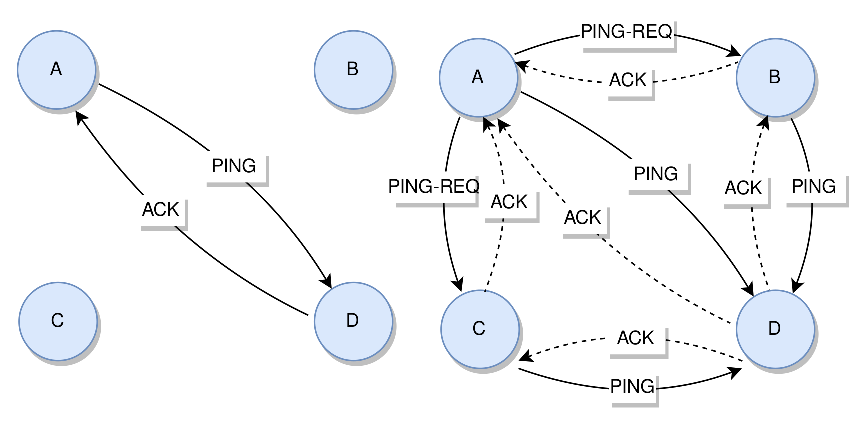
\includegraphics[scale=0.7]{images/Figure15}
	\end{center}
	\vspace{-0.6cm}
	\caption{Direct and indirect ping in SWIM protocol.}
	\label{fig:fig15}
\end{figure}

\noindent
Over the years, researchers found ways to improve the protocol, for example Dadgar et al. presented \textit{Lifeguard protocol}~\cite{DadgarPC18} for more accurate failure detection, and there are other implementations to fine-tune the SWIM, but the base idea is still there. Today SWIM or SWIM-like protocols are standard membership protocols whenever some node clustering is done.
%
%
\subsection{Mobile computing}\label{sec:mobile_computing}
%
The first idea that introduced task offloading from the cloud~\cite{FernandoLR13, LinLJL19} was Mobile cloud computing (MCC). Mobile devices run small client software and interact with the cloud over the internet, while heavy computation remains in the cloud. 

The cloud is usually far away from end devices because DCs are built on specific locations in the world to target as many users nearby as possible. This sparse deployment will most likely lead to high latency, and bad quality of experience (QoE)~\cite{LinLJL19} for most users. Latency-sensitive applications especially will have a hard time. As a model, MCC is not much different from the standard CC model. The good thing is that the cloud has been relaxed a little bit, and a small number of tasks has been moved from the cloud. But this model opens the door for the next-generation models.

The development led to new computing areas like EC, osmotic computig~\cite{VillariFDRJR19, VillariCF17}, sky computing~\cite{StoicaS21}, etc. EC is a next-generation model where computing and storage resources are in proximity to data sources~\cite{Satyanarayanan17}. This idea might overcome cloud latency issues and known MCC problems. The main strength of the EC lays in the CC enhancements with new processing ideas, for the next-generation use-cases~\cite{NingLSY20}. 

EC has brought a few different models over the years. Models like fog~\cite{BonomiMNZ14}, cloudlets~\cite{MonsalveCC18}, and mobile edge computing (MEC)~\cite{WangZZWYW17} emerged. This thesis will refer to all these models as edge nodes. Different EC models rely on the concept of data and computation offloading from the cloud closer to the ground~\cite{KhuneP19}. Only heavy computation remains in the cloud because of more available resources~\cite{NingLSY20}, compared to edge nodes. 

EC models introduced small-scale servers that operate between data sources and the cloud. These small-scale servers have much fewer capabilities compared to the cloud servers~\cite{ChenHLLW15}. To avoid latency and huge bandwidth~\cite{MonsalveCC18}, EC nodes can be dispersed in various locations, for example, base stations~\cite{WangZZWYW17}, coffee shops, or over arbitrary geographic regions.
%
%
\section{Distributed programming}\label{sec:distributed_computing}
%
DP can be defined as the use of a DS to solve one large problem, by breaking it down into several smaller parts, where each part is computed in the individual node of the DS and coordination is done by passing messages to one another~\cite{0019513}. Computer programs that use this strategy and run on top of the DS are called \textbf{distributed programs}~\cite{Vera16, andrews2000foundations}. 

Similar to CC in Section~\ref{sec:cloud_computing}, to a normal user, DC systems appear as a single system similar to one the user uses every day on his/her personal computer. DC shares the same fallacies to DS presented in~\ref{sec:distributed_systems}.
%
%
\subsection{Big Data}\label{sec:big_data}
%
Term big data means that the data is unable to be handled, processed, or loaded into a single machine~\cite{FisherDCD12}. That means that traditional data mining methods or data analytics tools developed for centralized processing may not be able to be applied directly to big data~\cite{Tsai2015}. 

New tools and methods that have been developed rely on DS and one specific feature \textbf{data locality}~\label{ds:data_locality}. Data locality can be described as a process of moving the computation closer to the data, instead of moving large data to computation~\cite{GuoFZ12}. This simple idea minimizes network congestion and increases the overall throughput of the system.

Two examples of how huge generated data could be have already been given in~\ref{sec:problem_area}, and when other IoT sensors and devices are included these numbers will just keep getting bigger and bigger~\cite{SarigiannidisLR20}.

Contrary to relational databases that mostly deal with structured data, Big Data is dealing with various kinds of data~\cite{FisherDCD12, Tsai2015, GuoFZ12}:

\begin{itemize}
	\item \textbf{Structured} data is a kind of data that have some fixed structure and format. A typical example of this is data stored inside a table of some database. Organizations usually have no huge problem extracting some kind of value out of the data.
	\item \textbf{Unstructured} data is a kind of data where there is not any kind of structure at all. These data sources are heterogeneous and may contain a combination of simple text files, images, videos, etc. This type of data is usually in raw format, and organizations have a hard time deriving the value out.
	\item \textbf{Semi-structured} data is the kind of data that can contain both previously mentioned types of data. An example of this type of data is XML files.
\end{itemize}

\noindent
Along with the share size, big data have other instantly recognizable features called \textbf{V's} of big data~\cite{PatgiriA16}. 

The name is derived from initial letters of the other features that are describing big data. 

Image~\ref{fig:fig3} show 6 V's commonly used to represent the big data.

\begin{figure}[H]
	\begin{center}
		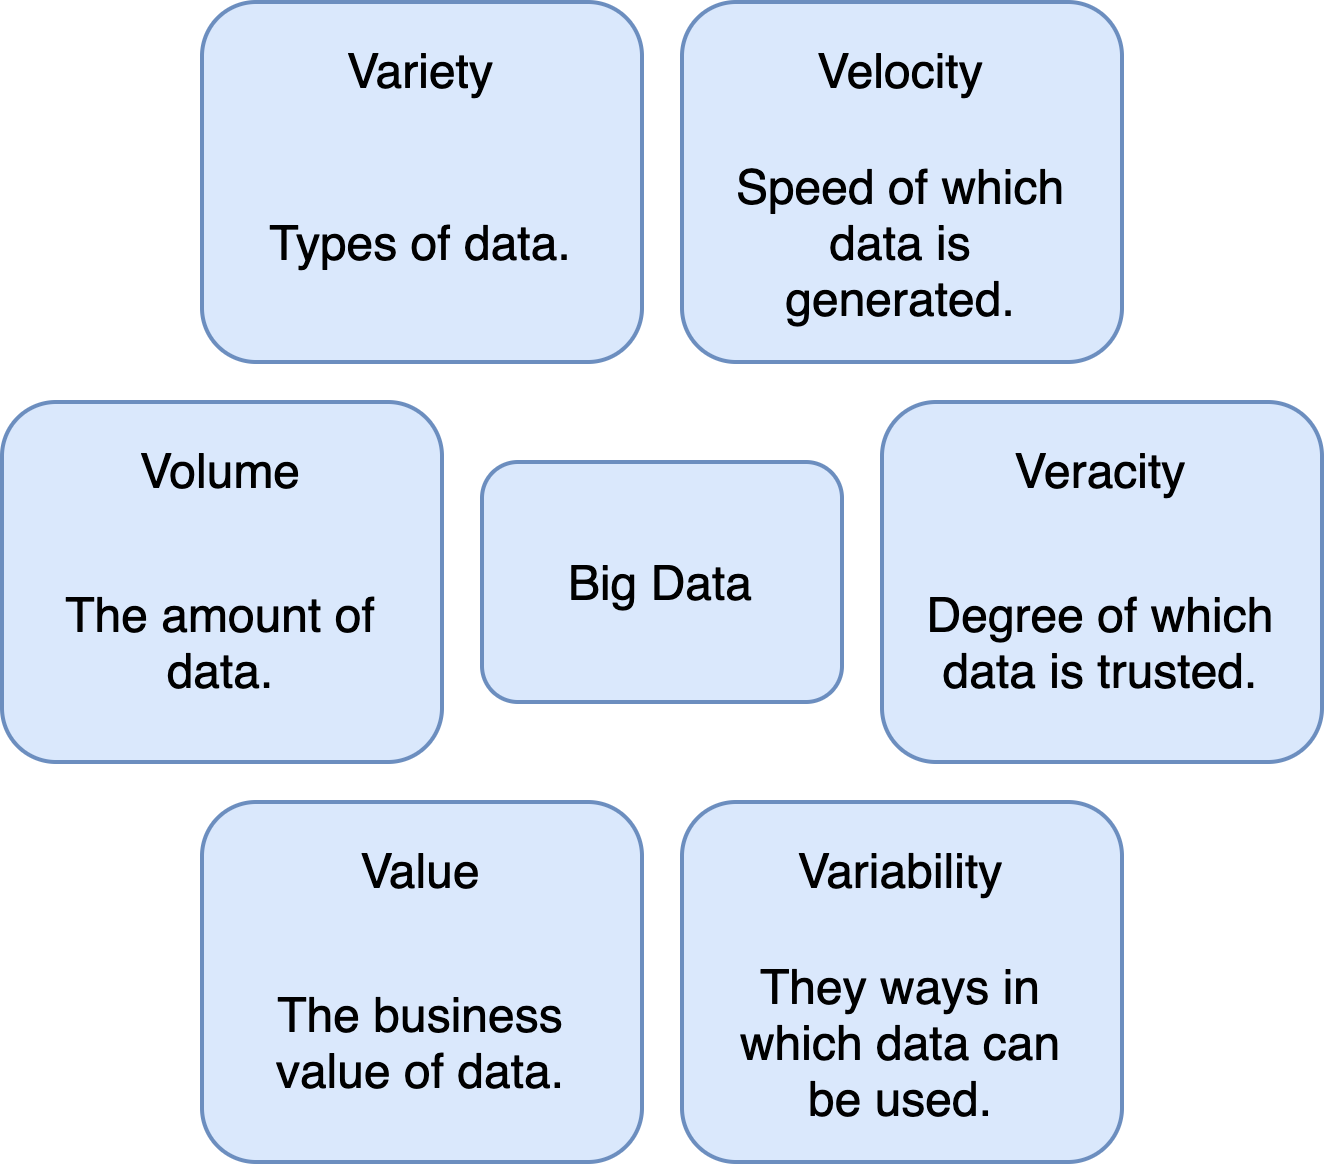
\includegraphics[scale=0.7]{images/Figure3}
	\end{center}
	\vspace{-0.6cm}
	\caption{V's of Big Data.}
	\label{fig:fig3}
\end{figure}

\noindent
Processing in big data systems can be represented as~\cite{phdthesis, KiranMMDB15}:

\begin{itemize}
	\item \textbf{Batch processing} represents a data processing technique that is done on a huge quantity of the stored data. This type of processing is usually slow and requires time.
	\item \textbf{Stream processing} represents a data processing technique that is done as data get into the system. This type of processing is usually done on a smaller quantity of the data \textbf{at the time}~\cite{medjedovic2022algorithms}, and it is faster.
	\item \textbf{Lambda architectures} represents a processing technique where \emph{stream processing} and handling of massive data volumes in a \emph{batch} are combined in a uniform manner, reducing costs in the process~\cite{KiranMMDB15}.
\end{itemize}

\noindent
Big data systems, are not processing and value extracting systems. Big data systems can be separated into several categories: \textbf{(1)} data storage, \textbf{(2)}, data ingestion \textbf{(3)}, data processing, and analytics. All these systems aid to properly analyze ever-growing requirements~\cite{RaoMBG19},

Despite a promise that big data offers to derive value out of the collected data, this task is not easy to do and requires a properly set up system filtering and removing data that contains no value. To aid this idea, data could be filtered and a little bit preprocessed on close to the source~\cite{inproceedingsSimic1}, and as such sent to data lakes~\cite{MarynowskiSP15}.
%
%
\subsection{Microservices}\label{sec:microservices}
%
There is no single comprehensive definition of what a microservice is. Different people and organizations use different definitions to describe it. A working definition is offered in~\cite{DragoniGLMMMS16} as~\say{a microservice is a cohesive, independent process interacting via messages}. Despite the lack of a comprehensive definition, all agree on a few features that come with microservices:

\begin{enumerate}[start=1,label={(\bfseries \arabic*)}]
	\item they are small computer programs that are independently deployable and developed.
	\item they could be developed using different languages, principles, and using different databases.
	\item they communicate over the network to achieve some goal.
	\item they are organized around business capabilities~\cite{PautassoZALJ17}.
	\item they are implemented and maintained by a small team.
\end{enumerate}

'\noindent
The industry is migrating much of their applications to the cloud because CC offers to scale their computing resources per their usage~\cite{LiZJLZLGGS19}. Microservices are small loosely coupled services that follow UNIX philosophy~\say{do one thing and do it well}~\cite{krause2015microservices}, and they communicate over well defined API~\cite{DragoniGLMMMS16}.

This architecture pattern is well aligned to the CC paradigm~\cite{LiZJLZLGGS19}, contrary to previous models like monolith whose modules cannot be executed independently~\cite{DragoniGLMMMS16, abs-1905-07997}, and are not well aligned with the CC paradigm~\cite{abs-1905-07997}. Table~\ref{tab:table3} summarizes differences between the monolith and microservices architecture.

\begin{table}[h!]
	\begin{center}
		\begin{tabular}{l|l|l}
			\textbf{Feature} & \textbf{Monolith} & \textbf{Microservices}\\
			\hline
			\textbf{Structure} & Single unit & Independent services \\
			\textbf{Management} & Usually easier & Add DS complexity\\
			\textbf{Scale/Update} & Entire app & Per service \\
			\textbf{Error} & Usually crush entire app & App continue to work \\
		\end{tabular}
	\end{center}
	\vspace{-0.5cm}
	\caption{Differences between the monolith and microservices architecture.}
	\label{tab:table3}
\end{table}

\noindent
Since its inception, microservices architecture has gone through adaptations, and modern-day microservices are extended with two new models, each with its unique abilities and problems:

\begin{itemize}
	\item \textbf{Cloud-native applications} are specially designed applications for CC. They are distributed, elastic, and horizontally scalable systems by their nature, and composed of (micro)services that isolate state in a minimum of stateful components~\cite{KratzkeQ17}. These type of applications are self-contained, could be deployed independently, and they are composed of loosely coupled microservices that are packaged in lightweight containers. They have Improved resource utilization, and they are centered around APIs.
	\item \textbf{Serverless applications} is a computing model, where the developers need to worry only about the logic for processing client requests~\cite{AdzicC17}. Logic is represented as an event handler that only runs when a client request is received, and billing is done only when these functions are being executed~\cite{AdzicC17}. \textbf{Cold start} is one of the features of serverless computing, and we can define it as user requests need to wait until a new container instance is up and running before it can do any processing at all. Most providers have 1–3 second cold starts, and this is important for certain types of applications where latency is a concern. Cold start is only happening when there are no \textit{warm} containers available for the request, meaning there is no single instance to server request. Other features include: \textbf{(1)} simplified services development, \textbf{(2)} faster time to market, \textbf{(3)} and lower costs.
	\item \textbf{Service Mesh} is designed to standardize the runtime operations of applications~\cite{LiLGZH19}. As a part of the microservices ecosystem, this dedicated communication layer can provide several benefits, such as: \textbf{(1)} observability, \textbf{(2)} providing secure connections, or \textbf{(3)} automating retries and backoff for failed requests. With these features, developers only focus on the implementation of business logic, while operators gain out-of-the-box traffic policies, observability, and insights from the services. Advocates of the microservice movement, nowadays recommend using service mesh architecture when running microservices in production environments.
\end{itemize}

\noindent
Previous models are not explicitly different, they all can be viewed as cloud-native applications. The enumeration is given for the sake of pointing out their different models and aspects of working.

Microservices communicate over a network to fulfill some goal using message passing techniques and technology-agnostic protocols such as HTTP. They can be implemented as:

\begin{itemize}
	\item Representational state transfer (REST) services~\cite{AdamczykSJH11}, is an architectural style with a set of constraints that users can create web services and interoperability between computer systems on the internet. It is based on HTTP routs to define resources and use HTTP verbs to represent operations over these resources. It relies on textual based communications, and payload could be represented using $JSON$, $XML$, $HTML$ etc.
	\item Remote procedure calls (RPC) represent an architectural way to design services that can call subroutines that are located in different places, usually on another machine. The client calls these operations like they are located locally in his address space.
	\item Event-driven services are services where communication between services is done using events. Events are sent on some channel and other read messages that are received on another channel. These channels could be implemented either like message queues or message topics. Services connect to message queue or subscribe to the specific topic, and when messages arrive, they can act according to the message type.
\end{itemize}

\noindent
They are well aligned with text-based protocols like HTTP/1 using $JSON$ for example, or binary protocols such as HTTP/2 using $protobuf$ and $gRPC$ for example, and even new faster version like HTTP/3 over new $QUIC$ protocol, designed by Google. HTTP/3 is the latest version of the conventional and trusted HTTP protocol. It is very similar to HTTP/2, but it also offers a few important new features. 

Table~\ref{tab:table9} shows important difference between versions of HTTP protocol.

\begin{table}[h!]
	\begin{center}
		\begin{tabular}{l|l|l|l}
			\textbf{Feature} & \textbf{HTTP1} & \textbf{HTTP2} & \textbf{HTTP3}\\
			\hline
			\textbf{Transport} & text & binary & binary\\
			\textbf{Parallelism} & No & Yes & Yes\\
			\textbf{Protocol} & TCP & TCP & QUIC \\
			\textbf{Space} & OS level & OS level & User level\\
			\textbf{Server push} & No & Yes & Yes\\
			\textbf{Compression} & Data & Data/Headers & Data/Headers\\
		\end{tabular}
	\end{center}
	\vspace{-0.5cm}
	\caption{Idempotent and non-idempotent operations.}
	\label{tab:table9}
\end{table}

\noindent
To ensure a wider range of devices that can communicate with the rest of the systems, developers usually have a gateway into the system that is REST service, and other services could be implemented differently.

It is important to point out, that all flavors of microservices applications rely on continuous delivery and deployment~\cite{7436659}. This is enabled by lightweight containers, instead of virtual machines~\cite{FelterFRR15}, and orchestration tools such Kubernetes~\cite{BurnsGOBW16}. These concepts will be described in more detail in Section~\ref{sec:virtualization_techniques}.

Microservices architecture is a good starting point especially for being built as a service applications model, and applications that should serve a huge amount of requests and users, especially with the benefits of CC to pay for usage, and the ability to scale parts of the system independently.  They are not necessarily easy to implement properly, and there is more and more critique to the architecture model~\cite{SoldaniTH18}. Microservices are rely upon and use parts of the DS, and as such, they inherit almost all problems DS has. 

One particular thing that users need to be aware of is \textbf{idempotency}. In microservices applications, developers are dealing with inconsistencies in the distributed state, and their operations should be implemented as idempotent. An operation is idempotent if it will produce the same results when executed over and over again. It is a strategy that means that operations with side effects like creation or deletion can be called any number of times while guaranteeing that side effects only occur once. Idempotency is a term that comes from mathematics, and can be represented by simple idempotency law for operation $*$ like~\cite{gratzer2002general}:

\begin{equation}\label{form:idempotency_law}
\forall x, x * x = x
\end{equation}
\myequations{Idempotency law formula}

\noindent
Not all Create, Read, Update, Delete (CRUD) operations are idempotent by default. Developers need to make effort to make all of them idempotent, to prevent bad outcomes and inconsistent states. 

Table~\ref{tab:table8} shows list of idempotent and non-idempotent for standard CRUD operations:

\begin{table}[h!]
	\begin{center}
		\begin{tabular}{l|c|c}
			\textbf{Operation} & \textbf{Idempotent} & \textbf{Non-idempotent}\\
			\hline
			\textbf{Create} &  & x \\
			\textbf{Read} & x & \\
			\textbf{Update} & x & \\
			\textbf{Delete} & x & \\
		\end{tabular}
	\end{center}
	\vspace{-0.5cm}
	\caption{Idempotent and non-idempotent operations.}
	\label{tab:table8}
\end{table}

\noindent
\emph{Crate} operation is \textbf{not} idempotent by default, but to make it idempotent there are multiple strategies how to do so. The most common way is to create \textbf{idempotency key} that will be sent in the request, and based on that request server can decide if this operation is already invoked or not. If a server has already \say{seen} specified idempotency key than the operation is already done and we can return just the response that the operation is done but no operation will be done over the state of the service or application. If the server sees the idempotency key for the first time, that is the signal that this request is a new one, and it should be done.

Idempotency key could be stored in any kind of storage, it is not uncommon that these keys are stored in cache storage with some time to live (TTL) policy that will automatically remove the key after a specified time.

Another option that is commonly used is hashing user specified actions. It is useful to know which part of the action set is already done and which is not. This strategy is used in scenarios where we must preserve the order of actions.
%
%
\subsubsection{Distributed Queries}~\label{sec:distributed_queries}
%
Applications built using microservices architecture propose different strategies for data storage. One common and recommended technique is \emph{database per service} patter~\cite{richardson2018microservices}.

The result of this technique is that overall state of the system will be distributed across multiple data stores, accessible only from their own microservices. This creates two important topics to think about: \textbf{(1)} transactions that span over multiple services can be implemented using \emph{Sagas} for example (cf.~\pageref{sec:sagas})
, and \textbf{(2)} the complex queries which require data from multiple databases.

The complex queries will involve data available in multiple databases, and a client can access all these microservices and aggregate data, however, this is not the recommended solution because the client does not have full understanding how the system manages the data.

In microservices archtiecture, there are two standard ways to solve this problem~\cite{richardson2018microservices}:

\begin{enumerate}
	\item \textbf{Command Query Responsibility Segregation (CQRS)}\label{par:cqrs} separates responsibility for \emph{modifying} data (command), and \emph{reading} the data (query), making the logic clearer and easier to optimize different parts of the system~\cite{richardson2018microservices, 8101372}. This increases the complexity of entire system, but it supports multiple denormalized views that are scalable and performant~\cite{richardson2018microservices}. 
	
	When the data in one service is modified, the service emits the event, which will change the service responsible for complex query. The service that will serve the queries will keep the \emph{read-only} replica of the data. 
	
	Figure~\ref{fig:fig21} shows an example diagram for CQRS pattern.
	
	\begin{figure}[H]
		\begin{center}
			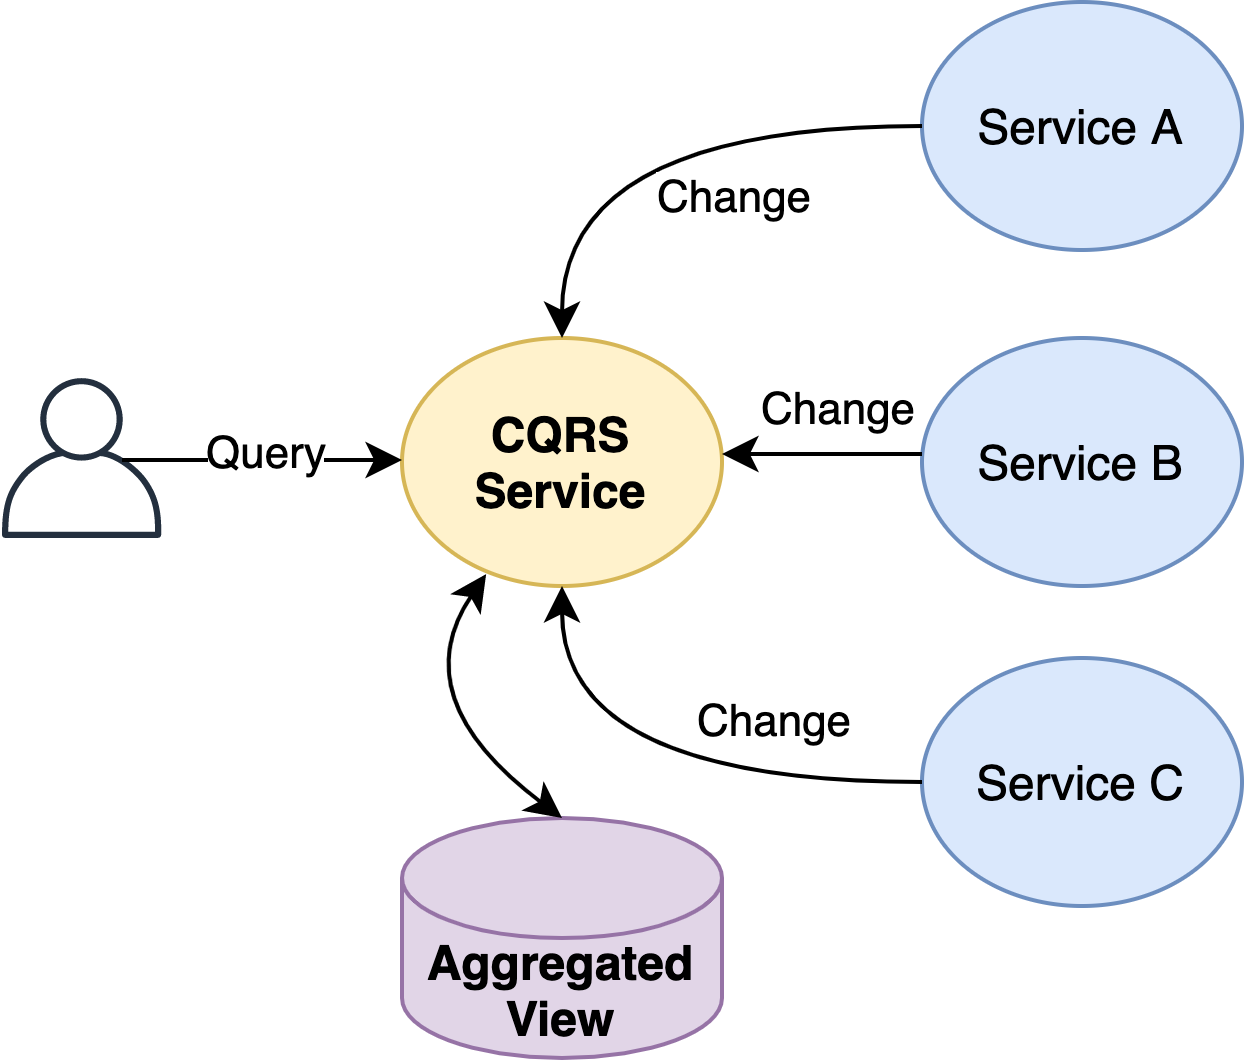
\includegraphics[scale=0.7]{images/Figure21}
		\end{center}
		\vspace{-0.6cm}
		\caption{CQRS pattern diagram.}
		\label{fig:fig21}
	\end{figure}

	\item \textbf{API composition}\label{par:composition} is a simple way to query data in a microservice architecture~\cite{richardson2018microservices, 8890660}, alternative and more lightweight solution than CQRS. 
	
	The main difference between CQRS is that this patterns does not have its own data storage. When a request comes in, it accesses every single microservice containing data, combines the results, and then returns the combined result to client. Making it easier to implement, because database does not need to be refreshed every time when some change occurs in the system. On the other hand, it may yield a slower response, depending on how many services we need to contact for the information, their availability, and time to merge and prepare data in memory. 

	Figure~\ref{fig:fig22} shows an example diagram for API Compossition pattern.

	\begin{figure}[H]
		\begin{center}
			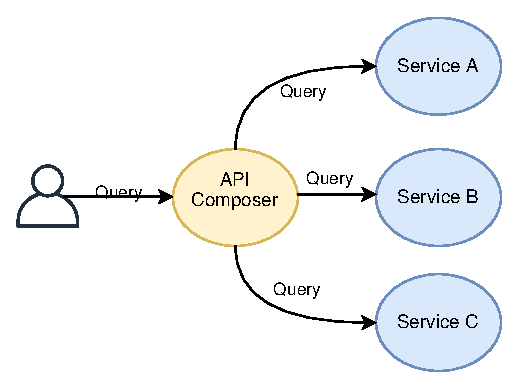
\includegraphics[scale=0.7]{images/Figure22}
		\end{center}
		\vspace{-0.6cm}
		\caption{API Compossition pattern diagram.}
		\label{fig:fig22}
	\end{figure}
\end{enumerate}

The best chance to succeed when implementing a microservices architecture is to simply follow existing patterns and use existing solutions with proven quality. 
%
%
\subsection{Observability}\label{sec:log_aggregation}
%
Observability is an integral part of any real-world computing system, and especially in the DS where observing what is happening in a network of processes is difficult~\cite{Fidge96}, due to the its nature.

In case of errors, fails or misbehavior of the system, some insight can be gained into what causes failure or which set of parameters in which circumstances. The three pillars of the observability are: \textbf{(1)} logs aggregation, \textbf{(2)} distributed tracing, and \textbf{(3)} alerting.

The logging operation, gives developers ability to store various arbitrary informations, that will provide more details for those who are investigating the failure. One thing we must be aware of is not to store any sensitive pieces of information in the log because this can cause a bunch of problems. Another thing we must be aware of is that we do not log too much and too often to slow down the business logic and execution of the function.

In monolithic applications logging and monitoring is a little bit easier to implement, because we have the whole application state in one place. When we come to the field of DS and microservices, our state is scattered across multiple elements or services. In DS, the monitoring involves interactions among concurrently executing processes~\cite{JoyceLSU87}.

The solution to this problem is to use a centralized logging service -- \textbf{logs aggregation}, that collects logs from each service~\cite{BeschastnikhWBE16}. This is beneficial because users can search and analyze the logs as a whole state of the system. To do this properly the log must be stored very reliably~\cite{DanielsST87}. Users can then configure the log server for some alerts that are triggered when certain messages appear in the logs. The log of DS usually does not contain enough information to regenerate the timeline of execution, and this is one reason that logs in DS are so hard to interpret~\cite{BeschastnikhWBE16}.

To resolve this problem of DS execution timeline, Google develops a new technique called \textbf{tracing}~\cite{36356}. The trace represents a single execution timeline or execution of one request. Trace will create a tree, and the tree is used to establish order. Every node in the tree represents a unit of work and it is called span. A tree unites all the elements needed to carry out an originating request. In every span or unit of work, we can attach more details about that particular execution element. 

Figure~\ref{fig:fig18} shows the simple example of \textit{RequestX} path through the processes in a distributed system, where each service \textbf{call} could be RPC, HTTP or some other request.

\begin{figure}[H]
	\begin{center}
		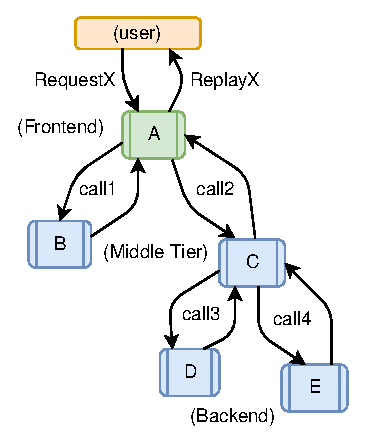
\includegraphics[scale=0.8]{images/Figure18}
	\end{center}
	\vspace{-0.75cm}
	\caption{\textit{RequestX} path through the processes in a distributed system.}
	\label{fig:fig18}
\end{figure}

\noindent
And last, but not the least option is \textbf{alerting}. Alerting of a monitored system can be represented as a set of rules that performs actions based on changes in specific metric. Alerting enables a system to notify users when something important happens or (probably) is going to happen.

DS logging, tracing and alerting represents the important role of any system, and as such, it should not be neglected especially in the DS environment. Every user request should be traced and logged from an infrastructure perspective, but we should allow users to store logs from their applications.
%
%
\section{Distribution Models}\label{sec:distribution_models}
%
The role of distribution models is to determine the responsibility for the request, or to answer the fundamental question \say{who is in charge} for a specific request. There are two ways to answer this question: \textbf{(1)} all nodes in the system, or \textbf{(2)} single node in the system.
%
%
\subsection{Peer-to-peer}\label{sec:p2p_networks}
%
Peer-to-peer (P2P) communication is a networking architecture model that partitions tasks or workloads between peers~\cite{Schollmeier01}. All peers are created equally in the system, and there is no such thing as a node that is more important than others. 

Every Peer has a portion of system resources, such as processing power, disk storage, or network bandwidth, directly available to other network participants, without the need for central coordination by servers or stable hosts~\cite{Schollmeier01}. P2P nodes are connected and share resources without going through a separate server computer that is responsible for routing. 

Figure~\ref{fig:fig2} shows difference in network topology between P2P networks $(left)$ and client-server architecture $(right)$.

\begin{figure}[H]
	\begin{center}
		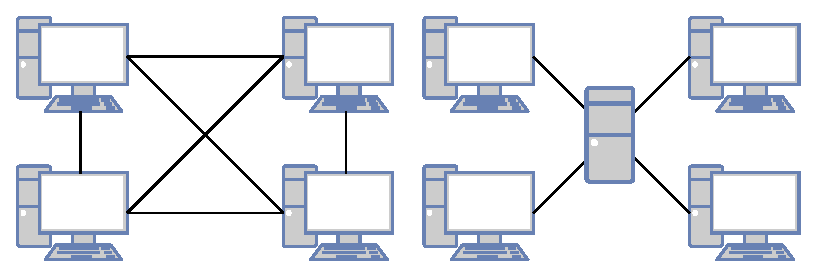
\includegraphics[scale=0.6]{images/Figure2}
	\end{center}
	\vspace{-0.6cm}
	\caption{P2P network and client-server network.}
	\label{fig:fig2}
\end{figure}

\noindent
Peers are creating a sense of virtual community. This community of peers can resolve greater tasks, beyond those that individual peers can do. Yet, these tasks are beneficial to all the peers in the system~\cite{BandaraJ13}. When a request comes to such a network, a node that accepts the request is usually called \textbf{coordinator}, because it then is trying to find the right peer to send a request to.

Based on how the nodes are linked to each other within the overlay network, and how resources are indexed and located, we can classify networks as~\cite{KamelSE07}:

\begin{itemize}
	\item \textbf{Unstructured} do not have a particular structure by design, but they are formed by nodes that randomly form connections~\cite{FilaliBHB11}. Their strength and weakness at the same time is the lack of structure. These networks are robust when peers join and leave the network. But when doing a query, they must find more possible peers that have the same piece of data. A typical example of this group is a Gossip-based protocol like~\cite{DasGM02}.
	\item \textbf{Structured} peers are organized into a specific topology, and the protocol ensures that any node can efficiently search the network for a resource. The famous type of structured P2P network is a Distributed Hash Table (DHT). These networks maintain lists of neighbors to do a more efficient lookup, and as such, they are not so robust when nodes join or leave the network. DHT is commonly used in resource lookup systems~\cite{StoicaMKKB01}, and as efficient resource lookup management and scheduling of applications, or as an integral part of distributed storage systems and NoSQL\cite{Leavitt10} databases.
	\item \textbf{Hybrid} combine the previous two models in various ways.
\end{itemize}

\noindent
P2P networks are a great tool in many arsenals, but because of their unique ability to act as a server and as a client at the same time, we must be careful and pay more attention to security because they are more vulnerable to exploits~\cite{0024003}.
%
%
\subsection{Master-slave}\label{sec:master_slave}
%
In the master-slave architecture, there is one node that is in charge -- \textbf{master}. This node accepts requests, and we usually do not communicate to the rest of the nodes or \textbf{slaves}. The master node is usually better and more expensive or even specialized hardware such as redundant array of inexpensive disks (RAID) to lower the crash probability. The cluster can also be configured with a \textbf{standby} master, and this node is continually updated from the master node.

But no matter how specialized hardware master runs on, it is prone to fail for various reasons, so it is a \textbf{single point of failure (SPOF)}. If crush happens, then standby master could continues to the server as a master, or new \textbf{leader election} protocol~\cite{KorachKM90} is initiated to pick a new master node. 

The master node is responsible for processing any updates to that data. If the master fails, then the slaves can still handle \textbf{read} requests. Failure of the standby master node to take over from the master node is a real problem if we want to achieve a high-availability system.

Figure~\ref{fig:fig16} shows difference between mater-slave $(left)$ and peer-to-peer $(right)$ request handling.

\begin{figure}[H]
	\begin{center}
		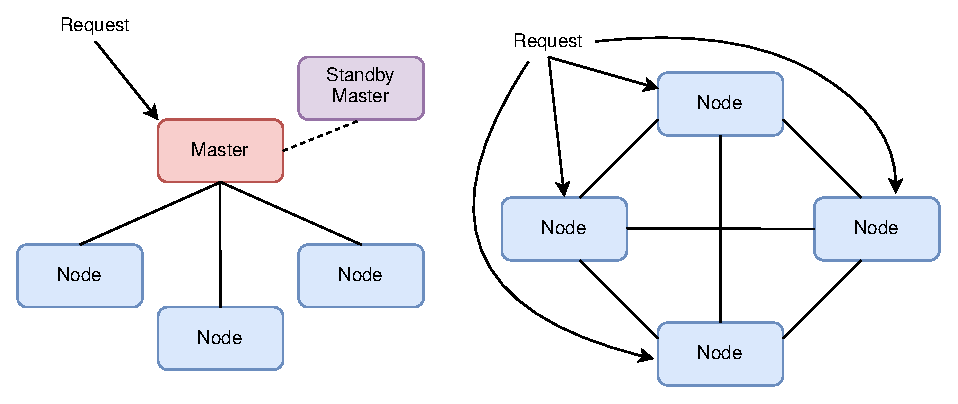
\includegraphics[scale=0.6]{images/Figure16}
	\end{center}
	\vspace{-0.6cm}
	\caption{Handling requests master-slave and peer-to-peer}
	\label{fig:fig16}
\end{figure}

\noindent
Using the right distribution model usually depends on the business requirements. High availability requires a P2P network because of no SPOF. If we could manage data using batch jobs that run in off-hours, then the simpler master-slave model might be the solution.
%
%
\subsection{Replication}\label{sec:replication_protocol}
%
Replication is a technique used to ensure the availability of redundant resources closer to the place where it is accessed, with a goal to improve reliability, fault-tolerance, or accessibility~\cite{SteenT16, 0019513}.

On the other hand, replication leads to better performance by balancing the load between components~\cite{SteenT16}. This is of importance, especially in geo-distributed systems, because it can lower down the communication latency. Users can access a copy of data nearby~\cite{0019513}.

Replication requires information about \textbf{replication factor}. The replication factor tells us the number of nodes to replicate the data. Replication could be implemented inside a single cluster or multiple regions, increasing the overall availability of the system further.

Storing data in several places requires that system deals with the \textbf{consistency} of stored data. The users can access different replicas at different times, leading the data to an inconsistent state. Consistency is tunable parameter, and user can choose between \textbf{strong} and \textbf{eventual} consistency.
%
%
\section{Similar computing models}\label{sec:similar_models}
%
In this section, we are going to shortly describe models that are similar to the DS, and as such, they may be the source of confusion.
%
%
\subsection{Parallel computing}\label{sec:parallel_computing}
%
DC and parallel computing seem like models that are the same, and that may share some features like simultaneously executing a set of computations in parallel. Broadly speaking, this is not far from the truth~\cite{Vera16}. 

Differencies between the two can be presented as follows: in parallel computing, all processor units have access to the shared memory and have some way of the faster inter-process communication, while in DS and DC all processors have their memory on their machine and communicate over the network to other nodes which are significantly slower. 

These models are similar, but they are not identical, and the kinds of problems they are designed to work on are different. Figure~\ref{fig:fig4} visually summarizes the architectural  differences between DC $(up)$ and parallel computing $(down)$.

\begin{figure}[H]
	\begin{center}
		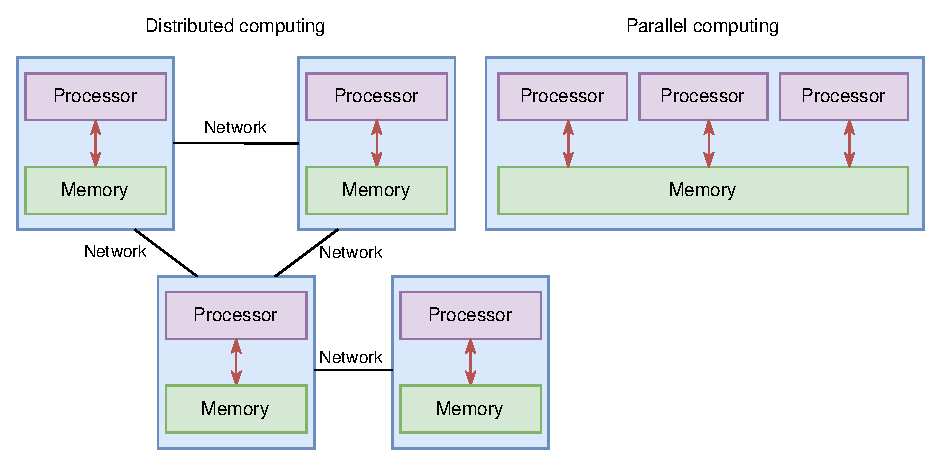
\includegraphics[scale=0.6]{images/Figure4}
	\end{center}
	\vspace{-0.6cm}
	\caption{Architectural difference between DC and parallel computing.}
	\label{fig:fig4}
\end{figure}

\noindent
Parallel computing has often used the strategy with problems that due to their nature or constraints must be done on multi-core machines simultaneously~\cite{0072397}. It is often that some big problems are divided into smaller ones, which can then be solved at the same time. 

Several tasks require parallel computing like simulations, computer graphics rendering, or different scenarios in scientific computing.
%
%
\subsection{Decentralized systems}\label{sec:decentralized_systems}
%
Decentralized systems are similar to DS, in a technical sense, they are still DS. But if we take a closer look, these systems \textbf{should not} be owned by a single entity. CC, for example, is a perfect example of DS, but it is not decentralized by its nature. It is a centralized system by the owner like AWS, Google, Microsoft, or some other private company because all computation needs to be moved to big DCs~\cite{HossainRH18}.

By modern standards, when we are talk about decentralized systems, we usually think of blockchain or blockchain-like technology~\cite{LeibleSSG19}, since here we have distributed nodes, that are scattered and there is no single entity that owns all these nodes. But even if this technology is run in the cloud, it is loses the decentralized feature. This is the caveat we need to be aware of. These systems are facing different issues because any participant in the system might be malicious and they need to handle this case. 

Nonetheless, CC can and should be decentralized in the sense that some computation can happen outside of cloud big DCs, closer to the sources of data. These computations could be owned by someone else, and big cloud companies could give their solution to this as well to relax centralization and problems that CC will have especially with ever-growing IoT and mobile devices.
%
%
\section{Transactions}\label{sec:transactions}
%
Transactions are keeping data consistent even in the presence of highly concurrent data accesses and despite all sorts of failures~\cite{WeikumV2002}. Transactions are trying to resolve this problem in a generic way, in such a way that is invisible to the application logic.

The main goal of transactions is to maintain system integrity in the consistent state, by ensuring that all operations on the system are either all completed successfully or all canceled successfully. Transactions are typically used in systems that needs to preserve some state (e.g. database or some filesystems). 

In their book Gray et al. make a good parallel with the contract law, saying that transactions give us the ability to \emph{clean up the situation}, if something does not work right.~\cite{GrayR93}.

Transactions guarantee following four properties: \textbf{(1)} atomicity, \textbf{(2)} consistency, \textbf{(3)} isolation, and \textbf{(4)} durability, also known as \emph{ACID} properties.
%
%
\subsection{Distributed transactions}\label{sec:distributed_transactions}
%
Because of the nature of DS, more network hosts are involved which significantly complicates the transaction mechanism. Distributed transactions are required to have all four \emph{ACID} properties. This might not be so easy to achieve amongst other due to \emph{CAP} theorem~\pageref{lab:cap}. 

In their book, Morgan et al. claim that here exists no distributed commit protocol that can guarantee independent process recovery in the presence of multiple failures (e.g., network partitionings)~\cite{WeikumV2002}.

Distributed transactions include few protocols such as two-phase commit (2PC), three-phase commit (3PC), Paxos, and various other approaches to quorum giving programmers facade of global serializability~\cite{Helland07}. 

Avoiding distributed transactions allows a much simpler, more robust and efficient solution.
%
%
\subsection{Sagas}\label{sec:sagas}
%
In 1987, Molina et al. presented \emph{Sagas}~\cite{Garcia-MolinaS87} and their work in the area of \emph{long-lived transactions (LLTs)}, types of transactions that hold resources for long periods, and as such delay shorter and more common transactions. 

These transactions are increasingly relevant and important, in the current technological landscape with the distribution of components and microservices architectures.

The saga transaction is composed of sub-transactions, executed in an atomic way so that either all or none of the sub-transactions take effect. However, no isolation is necessarily guaranteed between the sub-transactions of different sagas.

One transaction $T$ is composed of multiple sub-transactions $T_1,\ldots,T_n$, and every sub-transaction $T_i$ has an associated \emph{compensating transaction} $C_i$ or how the effects of the transaction can be rolled back. The saga transaction executes sub-transactions sequentially.

Figure~\ref{fig:fig20} shows an example of one transaction separated into multiple sub-transactions where \emph{green} arrows represent success path, while \emph{red} arrows represent rollbacks, structure of the saga transaction and at least the previous and next element in the chain.

\begin{figure}[H]
	\begin{center}
		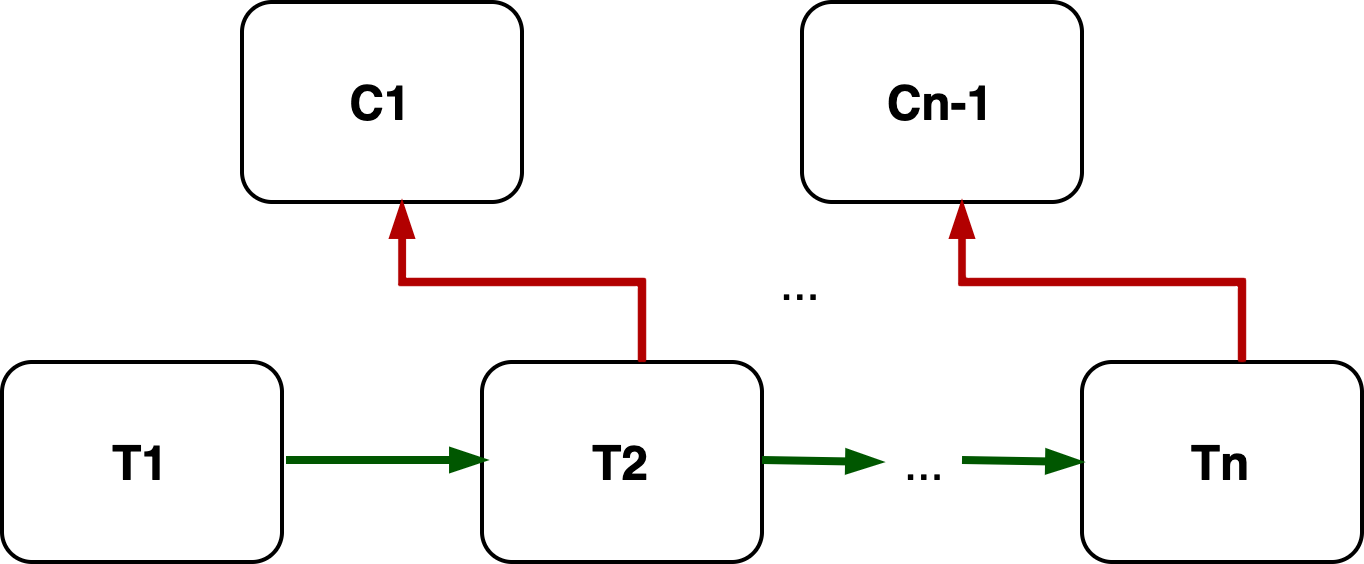
\includegraphics[scale=0.8]{images/Figure20}
	\end{center}
	\vspace{-0.6cm}
	\caption{Saga transactions separated in sub-transactions.}
	\label{fig:fig20}
\end{figure}

\noindent
Sagas can be implemented using two patterns: \textbf{(1)} orchestration where one centralized element is responsible for all the coordinating, or \textbf{(2)} choreography, where each service trigger local transactions in other services.

This isolation can be added in the application layer~\cite{Frank}l for example using \emph{semantic lock}. This strategy will change state so that some data are in process and should be treated differently. 

For example, an order can be in one of the following states: \textbf{(1)} \emph{PENDING}, \textbf{(2)} \emph{COMPLETED}, or \textbf{(3)} \emph{CANCELED} state. Other transactions will not make use the data if status is not set to \emph{COMPLETED}.
%
%
\section{Garbage collection}\label{sec:garbage_collection}
%
Most modern programming languages nowadays allow programmers to allocate and free memory. This process can be in total responsibility of the programmer, or language can handle this process for the programmer. When there is some automatic process involved to release unused resources, that process is called \textbf{garbage colection} or GC. 

In~\cite{JonesL96}, Jones, et al. describe \emph{garbage collection} as the automatic management of dynamically allocated storage. However, the term \emph{garbage collection} is not exclusive to programming languages. It is widely used to refer to all forms of automatic management of dynamically allocated resources.

Even with the rapid growth of memory sizes, and lowering the overall cost of memory is not inexhaustible. Like any other limited resources, it requires careful consideration and recycling. Even tools like Kubernetes, have some form of garbage collection that is used to remove unused items and their references in the system.

Over the years, different algorithms are used to do reference counting and tracing methods, to discover unused resources, and to free them. One of the most common algorithms for garbage collection is \emph{mark-sweep} algorithm~\cite{McCarthy60} developed in 1960. The variety on the topic exists today, but the essence of the algorithm remains widely used today.

Traditional automated garbage collection is usually seen as slow, and disruptive to executing programs. Modern implementations of the garbage collection substantially reduced the overhead of the system~\cite{JonesL96}.
%
%
\section{Virtualization techniques}\label{sec:virtualization_techniques}
%
Virtualization as a technique started long ago in time-sharing systems, to provide isolation between multiple users sharing a single system like a mainframe computer~\cite{CrosbyB06}. 

In~\cite{Sharma} Sharma et al. virtualization is described as technologies that provide a layer of abstraction of the physical computing resources between computer hardware systems and the software systems running on them.

Modern virtualization differentiates several different tools. Some of them are used as an integral part of the infrastructure for some flavors like IaaS, while others are used in different CC flavors as well as microservices packaging and distribution format, or are new and still are looking for their place. These options are:

\begin{itemize}
	\item \textbf{Virtual machines (VM)} are the oldest technology of the three. They are described as a self-contained operating environment consisting of guest operating system and associated applications, but independent of the host operating system~\cite{Sharma}. VMs enable us to pack isolation and better utilization of hardware in big DCs. They are widely used in IaaS environment~\cite{AbsalomBJ13, YangHCLW13} as a base where users can install their own operating system (OS) and require software tools and applications.
	\item \textbf{Containers} provide the almost same functionality to VMs, but there are several subtle differences that make them a go-to tool in modern development. Instead of the guest OS running on top of host OS, containers use tools that are in a Linux kernel like \textit{cgroups} that limit process resource usage so that single process can not starve other processes and use all the resources for itself, and \textit{namespaces} to provide isolation and partitions kernel resources so that single process sees node resources like it only exists there. Containers reduce time and footprint from development to testing to production, and they utilize even more hardware resources compared to VMs and show better performance compared to the VMs~\cite{Seo2014PerformanceCA, FelterFRR15}. Containers provide an easier way to pack services and deploy and they are especially used in microservices architecture and service orchestration tools like Kubernetes~\cite{BurnsGOBW16}. Google has stated several times in their online talks that they have used container technology for all their services, they even run VMs inside containers for their cloud platform. Even though they exist for a while, containers get popularized when companies like Docker and CoreOS developed user-friendly APIs.
	\item \textbf{Unikernels} is the newest addition to the virtualization space. Unikernels are defined as small, fast, secure virtual machines that lack operating systems~\cite{pavlicek2016unikernels}. Unikernels are comprised of source code, along with only the required system calls and drivers. Because of their specific design, they have a single process and they contain and execute what it absolutely needs to nothing more and nothing less~\cite{GoethalsSAVT18}. They are advertised as new technology that will save resources and that they are \textit{green}~\cite{208735}, meaning they save both power and money. When put to the test and compared to containers they give interesting results~\cite{GoethalsSAVT18, PlauthFP17}. Unikernels are still a new technology and they are not widely adopted yet. But they give promising features for the future, especially \textbf{if} properly ported to ARM architectures, and various development languages. Unikernels will probably be used as a user application and function virtualization tool, because of their specific architecture, especially for serverless applications presented in~\ref{sec:microservices}.
\end{itemize}

\noindent
With every virtualization technique, the ultimate goal is to pack as many applications on existing hardware as possible, so that there are no resources that are left not used -- we are trying to achieve high resource utilization. 

Figure~\ref{fig:fig5} represents architectural differences between VMs, containers, and unikernels.

\begin{figure}[H]
	\begin{center}
		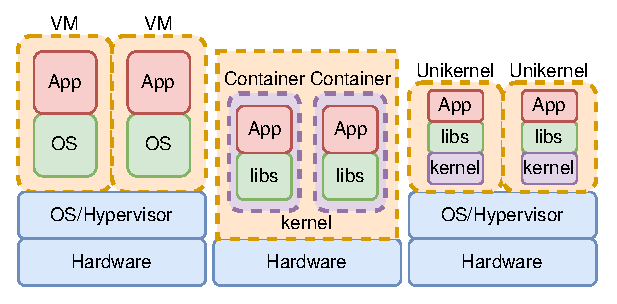
\includegraphics[scale=0.80]{images/Figure5}
	\end{center}
	\vspace{-0.6cm}
	\caption{Architectural differences between VMs, containers and unikernels.}
	\label{fig:fig5}
\end{figure}
%
%
\section{Deployment}\label{sec:deployment}
%
Over the years different approaches evolved how to deploy infrastructure and applications. The difference just gets more amplified, when CC and microservices get into the picture, where frequent deployment is very common. 

Deployments in such complex environment can be separated by how they handle changes on existing infrastructure or applications on:

\begin{itemize}
	\item \textbf{A mutable model} is a model where we have in place changes which mean that the parts of the existing infrastructure or applications get updated or changed to do an update. In place change can produce some problems, and has:
	
	\begin{enumerate}[start=1,label={(\bfseries \arabic*)}]
		\item more risk because in-place change may not finish, which puts our infrastructure or the application in a possible bad state. This is especially a problem if we have a lot of services and multiple copies of the same service. The possibility that our system is not on is a lot higher.
		\item high complexity, this is a direct implication of the previous feature. Since our change might not get fully done, it cannot be guaranteed that our infrastructure or application is transitioned from one version to another -- change is not \textbf{discrete}, but \textbf{continues} since we might end up in some state in between where we are now and where we want to be.
	\end{enumerate}
	
	\item \textbf{An immutable model} is a model where no in-place changes on existing infrastructure or application are done whatsoever. In this model, the previous version is replaced completely with a new version that is updated or changed compared to the previous version. The previous version gets discarded in favor of the new version. Compared to the previous model, immutable deployment:
	
	\begin{enumerate}[start=1,label={(\bfseries \arabic*)}]
		\item has less risk, since the existing infrastructure or the application, is not changed, but a new one is started and the previous one is shut down. This is important especially in DS where everything can fail at any time.
		\item has less complexity of the mutable deployment model. This is a direct implication of the previous feature since the previous version is shut down and fully replaced with the new one. This is a \textbf{discrete} version change and atomic deployment with deferring deployments with fast rollback and recovery processes.
		\item requires more resources~\cite{Helland16}, since both versions must be present on the node for this process to be done. The second problem is the data that the application has generated should not be lost. The problem is solved by externalizing the data. We should not rely on local storage but store that data elsewhere, especially when the parts of the system are volatile and changed often. The key advantage of this approach is avoiding downtime experienced by the end-user when new features are released. 
	\end{enumerate}
\end{itemize}

Immutability is a simple concept to understand and simplifies a lot especially in DS~\cite{Helland16}. Write down some data, and ensure that it never changes. It can never be modified, updated, or deleted~\cite{perry2020art}. When this is combined with the promise that downtime can be avoided especially in complex DS, it is clear why the immutable model is gaining more and more popularity (especially with the arrival of containers). 

Immutable infrastructure deployment offers several benefits on how to deploy changes. Even in production, it is easier to switch to a whole new version. These strategies include:

\begin{itemize}
	\item \textbf{Blue-Green deployment}, this strategy requires two separate environments: \textbf{(1)} \textit{Blue} current running version, and \textbf{(2)} \textit{Green} is the new version that needs to be deployed. When there is satisfaction that the green version is working properly, the traffic can be gradually rerouted from the old environment to the new one,  for example by modifying the Domain Name System (DNS). This strategy offers near-zero downtime.
	\item \textbf{A canary update} is a strategy where a small subset of requests is directed to the new version --- the canary, and the rest of them are directed to an old version. If the change is satisfactory, the number of requests can be increased, and it should be monitored how the service is working with increasing load, if there are errors, etc.
	\item \textbf{Rolling update} strategy updates large environments, a few nodes at the time. The setup is similar to blue-green deployment, but here there is a single environment. With this strategy, the new version gradually replaces the old one. If for whatever reason the new version is not working properly on the larger number of nodes, rolling back to the previous version can always be done.
\end{itemize}

\noindent
With mutable infrastructure, these strategies would be hard to implement, and maybe it is not possible at all. Besides infrastructure deployment, there is another side that we must be considered, and that is how to describe these deployments. Two different strategies can be considered here:

\begin{itemize}\label{lab:dep_types}
	\item \textbf{Imperatively}, with this option users have to write code or specific instructions step by step what the specific tool needs to do so that the application or infrastructure is properly set up. In this approach, we have a \textit{smart} user who describes \textit{dumb} machine what is needed to be done and in what order to achieve the desired state.
	\item \textbf{Declaratively}, with this option a user has to describe the end state or what is his desired state, and the tool needs to figure out the way how to do this. Here we have a \textit{smart system} that will find a way how to achieve the \textbf{desired state}, and we have a user who\textit{does not care} in what order actions need to be done --- that is what the system needs to do. Users do not need to worry about timing, this simplifies the whole process and the code always represents the latest state. With this type of deployment, we can offer users, two different models:
	
	\begin{enumerate}[start=1,label={(\bfseries \arabic*)}]
		\item using existing platform independent formats that users are familiar with, like \textit{JSON, YAML, XML}, etc.
		\item using a domain-specific language (DSL) that users need to learn, but we might be able to optimize description.
	\end{enumerate}
\end{itemize}

\noindent
So far, the first option is preferred by many companies, because users are already familiar with these formats, and does not require developers time to develop new DSL. If the platform becomes too complicated then it makes sense to develop DSL for this purpose.

Figure~\ref{fig:fig12} summarizes the difference between mutable and immutable deployment models.

\begin{figure}[H]
	\begin{center}
		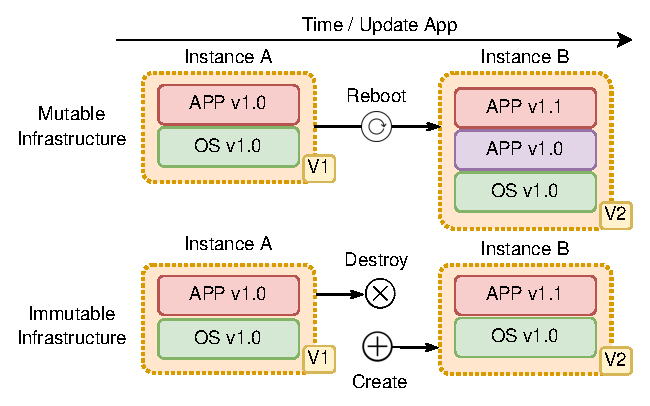
\includegraphics[scale=0.80]{images/Figure12}
	\end{center}
	\vspace{-0.6cm}
	\caption{Difference between mutable and immutable deployment models.}
	\label{fig:fig12}
\end{figure}

\noindent
With the introduction of \textit{LinuxKit}, Linux subsystems are based around very secure containers. With LinuxKit, every part of the Linux subsystem runs inside the container, so a Linux subsystem can be assembled with services that are needed. As a result, systems created with LinuxKit have a smaller attack surface~\cite{abs-1802-10375} than general-purpose systems. 

This is important not only from the security point of view but also for infrastructure deployment as well. Specific OSs can be created, based on the containers for a different purpose. They can be updated, changed, and adapted for every machine or purpose needed.

Deployment is based on changing parts of the OS, and services that run inside the containers. As a result, everything can be removed or replaced. It's highly portable and can work on desktops, servers, IoT, mainframes, bare metal, $\upmu$DCs at the edge, and virtualized systems.

\section{Infrastructure as software}~\label{sec:ias}
%
The infrastructure needs to be constantly deployed and maintained, so it would be beneficial to view the infrastructure as software (IaS)~\cite{Fitzgerald}. The benefit of this approach lies in the already available tools, principles, and techniques (e.g. reuse, testing, modeling, and evaluation) that can equally be used for the infrastructure definitions ~\cite{Osterweil, Fitzgerald}.

In his work~\cite{Osterweil}, Osterweil et al. argue that software and software processes share some similar characteristics: \textbf{(1)} both are executed, \textbf{(2)} both have requirements that need to be understood, \textbf{(3)} both benefit from being modeled, and \textbf{(4)} both can be guided by measurement.

Fitzgerald et al.~\cite{Fitzgerald} argue that process programming, defined by Osterweil~\cite{Osterweil} et al., is applicable in the infrastructure domain. The authors claim that it is useful to extend the “software process as software” paradigm to include infrastructure as software (IaS). The move towards multi-tier systems that involve cloud and cyber-physical systems will only stimulate the connection between software and reliable infrastructure systems.

Looking at the infrastructure configuration as the software allows application developers to venture into the “infrastructure programming”~\cite{Fitzgerald}, allowing platforms and infrastructure to be managed in a similar way as the software is.

In a cloud environment, it is an essential technique to properly implement continuous deployment, giving us tools to automate the configuration and provisioning process of infrastructure using cloud instances~\cite{RahmanMW19}. Wittig et al. describe it as a process of managing and provisioning computer data centers through machine-readable definition files, rather than physical hardware configuration or interactive configuration tools~\cite{wittig2018amazon}. 
%
%
\subsection{Infrastructure as code}
%
In modern cloud and microservices era, a new strategy to manage and deploy complicated infrastructure elements -- Infrastructure as code (IaC). In his book~\cite{wittig2018amazon} Wittig et al. describe it as a process of managing and provisioning computer data centers through machine-readable definition files, rather than physical hardware configuration or interactive configuration tools. 

IaC has grown in popularity in recent years because it applies the same kind of version control and repeatability to the orchestration of the infrastructure as developers use for applications source code~\cite{ArtacBNGT17}. The second benefit is that configuration is decoupled from the system, it can more readily be deployed on a similar system elsewhere. 

IaC is a continuation of earlier works of Osterweil et al.~\cite{Osterweil}, and Fitzgerald et al.~\cite{Fitzgerald}, trying to move infrastructure to level of software, keeping existing tools, best practices and techniques. It relys on the \textbf{reconciler pattern}~\cite{luksa2018kubernetes}, widely used in scheduling systems like Kubernetes.

This pattern enables tracking of resources using two simple states:~\label{loop_pattenr} 

\begin{enumerate}[start=1,label={(\bfseries \arabic*)}]
	\item \textbf{expected state} represents the desired state provided by the user. This is the state that must be (if possible) achieved at any give point in time;
	\item \textbf{current state} refers to the actual system state. This state must be refreshed periodically, so that system know should it be corrected or not.
\end{enumerate}

\noindent
The reconciler pattern runs a \textbf{reconciliation loop} that ensures that the \emph{current state} remains the same as the \emph{expected state}.~\label{reconcile_loop} 

Figure~\ref{fig:fig26} presents reconciliation loop diagram.

\begin{figure}[H]
	\begin{center}
		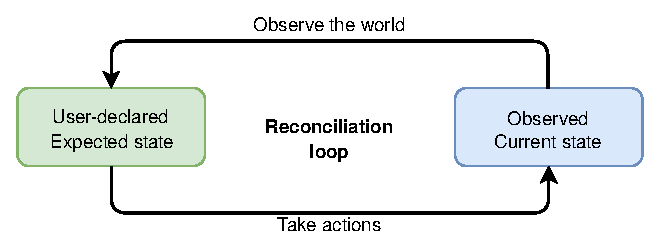
\includegraphics[scale=0.80]{images/Figure26}
	\end{center}
	\vspace{-0.6cm}
	\caption{Reconciliation loop diagram.}
	\label{fig:fig26}
\end{figure}

Every node must provide its current state regularly, and when some state is divergent from the desired state, the system must act to ensure that this situation is corrected automatically. The node can send its state over existing channels e.g., \textbf{health-check} pings to minimize load and data transferred over the network, or a dedicated channel just for this purpose may exist.

Extension of such system can be done just by writing new \emph{controller} that will react on changes for newly added kind of workload.
%
%
\section{Development roles}\label{sec:dev_roles}
%
In our modern internet-connected world of applications, we have several distinctive development roles. Each of them plays an important role so that modern software runs smoothly, and with less downtime. These development roles could be separated into a few categories (focus is on the technical roles):

\begin{itemize}
	\item \textbf{A developer} is usually a person responsible for developing software for the user. A developer is responsible for maintaining existing, and/or developing new features. There could be different sub-roles, dealing with specific parts of the complex software systems.
	\item \textbf{DevOps} role represents a multidisciplinary organizational effort to automate application deployments through continuous delivery of new software updates~\cite{LeiteRKMM20}. It combines software development with technology operations~\cite{JabbariAPT16} to shorten the development life cycle.
	\item \textbf{Site Reliability Engineer (SRE)} role is responsible for availability, latency, performance, efficiency, change management, monitoring, emergency response, and capacity planning~\cite{beyer2016site}. It is a software engineering role and needs to have an understanding of the fundamentals of computing~\cite{JonesUN15}, applied to the infrastructure and operations problems.
\end{itemize}

\noindent
DevOps and SREs seem to be similar roles, they are both trying to bridge the gap between development and operations. As such they have a very large conceptual overlap in how they operate~\cite{46939}, but also have some differences. 

Table~\ref{tab:table10} sums the differences between the DevOps and SREs.

\begin{table}[H]
	\begin{center}
		\begin{tabular}{l|ll}
			\textbf{Feature} & \textbf{DevOps} & \textbf{SREs}\\
			\hline
			\textbf{Task} & \multirow{2}{10em}{Scaling, uptime, robustness} & \multirow{2}{10em}{Development pipeline} \\
			& & \\
			\textbf{Essence} & Practices and metrics &  Mindset and culture \\
			\textbf{Team structure} & \multirow{3}{10em}{Wide range of roles: QA, developers, SREs etc.} &  \multirow{3}{10em}{SREs with operations and development skills} \\
			&  &  \\
			&  &  \\
			\textbf{Focus} & \multirow{2}{10em}{Development and delivery continuity} & \multirow{2}{10em}{System availability and reliability} \\
			&  &  \\
			\hline
			\textbf{Goal} & \multicolumn{2}{c}{\multirow{2}{12em}{Bridge the gap between development and operation}} \\
			&  &  \\
		\end{tabular}
	\end{center}
	\vspace{-0.5cm}
	\caption{Differences between DevOps and SREs.}
	\label{tab:table10}
\end{table}

\noindent
In modern complex software development, SREs should keep things running smoothly, while DevOps principles should be used to improve processes. 

So it is not either/or, but it seems that a combination of approaches may provide the best results. However, in some smaller organizations, these roles can overlap.
%
%
\section{Concurrency and parallelism}\label{sec:concurency_parallelism}
%
People usually confuse these two concepts. Even though look similar, they are a different way of doing things. In his speech, Rob Pike~\cite{Pike} gives a great explanation and examples on this topic. He also gives great definitions of these concepts like:

\begin{itemize}
	\item \textbf{Concurrency} is composition of independently executing things. Concurrency is about dealing with a lot of things at once.
	\item \textbf{Parallelism} is the simultaneous execution of multiple things. Parallelism is about doing a lot of things at once. 
\end{itemize}

\noindent
These things are important, especially when building applications and systems that should achieve very high throughput. They must be built with a good structure and a good concurrence model. These features enable possible parallelism, but with communication~\cite{Pike}. These ideas are based on Tony Hoare work of Communicating Sequential Processes (CSP)~\cite{Hoare78}.

\subsection{Actor model}\label{sec:actor_model}
%
An actor model, the main idea is based around \textbf{actors} which are small concurrent code, that communicate independently by sending messages, removing the need for lock-based synchronization~\cite{Hewitt}. This model proposes a similar idea to Tony Hoare's in his work with CSP~\cite{Hoare78}, and actors are often confused with CSP. 

Table~\ref{tab:table6} gives differences between an actor model and CSP.

\begin{table}[h!]
	\begin{center}
		\begin{tabular}{l|l|l}
			\textbf{Feature} & \textbf{CSP} & \textbf{Actor model}\\
			\hline
			\textbf{Fault tolerance} & Distributed queue &  Supervisors hierarchy \\
			\textbf{Process identity} & Anonymus & Concrete \\
			\textbf{Composition} & Not applicable & Applicable \\
			\textbf{Communication} & Queue & Direct \\
			\textbf{Message passing} & Sync & Async\\
		\end{tabular}
	\end{center}
	\vspace{-0.5cm}
	\caption{Differences between actor model and CSP.}
	\label{tab:table6}
\end{table}

\noindent
Actors do not share a memory, and they are isolated by nature. An actor can create another actor/s and even watch on them in case they stop unexpectedly. When an actor finished its job, and it is not needed anymore, it disappears. These actors can create complicated networks that are easy to understand, model, and reason about, and everything is based on a simple message passing mechanism. 

Every actor has a designated message box. When a message arrives, the actor will test the message type and do the job according to the message type he received. In this way, we are not dependent on lock-based synchronization that can be hard to understand, and it can cause serious problems.

The actor model is fault-tolerant by design. It supports crush to happen because there is a \say{self-heal} mechanism that will monitor actor/s, and when the crash happens it will try to apply some strategy, in most cases just restart actor, but other strategies could be applied. This philosophy is useful because it is hard to think about every single failure option.
%
%